Transaction throughput is a key benchmark for the performance of transactional
databases. Systems with stronger isolation levels tend to have lower transaction
throughout resulting from the increased number of aborted transactions.
Therefore, in this experiment, transaction throughput is used to determine the
performance impact of serializability in NVRAM-based key-value stores.

\subsubsection{Setup}

In order to perform this experiment, one not only needs data to work on but also
a set of concrete transactions and the operations they are composed of, i.e. a
workload. As with data, it is hard to acquire actual transaction traces and
determine their relevance. For that reason, the experiment setup relies heavily
on randomly generated data. However, each random choice is reproducible as the
generated data are stored on disk prior to the experiment. Hence, the only
non-deterministic behaviour is induced by multi-threading, the operating system,
and the underlying hardware.

\paragraph{Data}

For uniformity, this experiment uses the exact same sets of random key-value
pairs that are used in Chapter \ref{ch:eval-baseline}. Thus, there is one data
set with 1K entries and another with 100K entries. When the experiment starts,
each individual KVS will be populated with these key-value pairs.

\paragraph{Workloads}

All transactions that are to be executed during the experiment are encoded as a
workload. A workload specifies for each transaction its operations and the
respective key-value pairs to operate on. When generating a workload, there are
three important dimensions:

\begin{itemize}
    \item length of transactions
    \item number of transactions
    \item relative distribution of operations
\end{itemize}

The length of a transaction is the number of operations enclosed in that
transaction. Intuitively, the length of transactions should vary. Unfortunately,
no reliable sources as to the absolute quantities of transaction lengths could
be found. As a result, the following ranges are deemed meaningful:

\begin{figure}[!h]
    \centering
    \begin{tabular}{|l|l|l|}
        \hline
        \textbf{Name} & \textbf{Min. No. Ops} & \textbf{Max. No. Ops} \\
        \hline
        Short         & 2  & 32  \\
        Long          & 64 & 256 \\
        \hline
    \end{tabular}
    \caption{Types of transactions in terms of length.}
    \label{tab:tx-length}
\end{figure}

Short transactions can be small updates like incrementing a numeric value,
optionally based a small aggregation. Long transaction on the other hand, can be
larger aggregations such as computing a sum over many items.

When specifying the operations of a transaction, it must be decided whether an
operation reads or updates an item. Insert and delete operations are omitted as
they complicate the experiment when run concurrently. For example, a concurrent
transaction might fail because an expected pair has not been inserted yet. Such
an incident reduces transaction throughput without an actual conflict which
could distort results. The remaining two operations are selected based on the
empirical analysis in \cite{andrei2017sap}. According to the source, read
operations amount of 84\% of all operations. The remaining 16\% are sumsumed as
updates for this experiment. Each operation acts on keys from the dummy set that
are selected randomly during the workload generation. All pseudo-random numbers
were generated using uniform distributions based on seperate mersenne twister
engines. Each workload consists of 1000 transactions.

\paragraph{Scenarios}

Resulting from the dimensions shown above, four unique scenarios  were derived:

\begin{itemize}
    \item S1: small database, short transactions
    \item S2: small database, long transactions
    \item S3: large database, short transactions
    \item S4: large database, long transactions
\end{itemize}

These scenarios are supposed to simulate both low and high contention in
different forms. In a database that is small compared to the number of
concurrent transactions, it is very likely that multiple transactions operate on
the same data which can cause conflicts. Likewise, longer transactions cause
contention as they are more likely to access data of other transactions. That
said, scenario 1 and especially scenario 2 simulate high contention which is the
worst-case for any concurrency control. The reason is that contention often
causes conflicts which lead to aborts and reduced transaction throughput. With
larger databases, short transactions are less likely to access the same data
which reduces contention. However, as transactions become longer, they become
more likely to collide and abort.

\subsubsection{Procedure}

The benchmark is performed separately for each KVS. The general procedure is to
execute each workload with a different number of cores. Since the underlying
machine has 32 physical cores, the experiment is performed with 1, 2, 4, 8, 16,
and 32 cores. During each run, several statistics such as the total time taken
and the number of aborts are captured. In order to reduce the influence of
outliers, each run, i.e. a combination of workload and core count, is performed
10 times. As a result, for each store there is a total of 24 configurations
which amounts to a total of 480 runs including repetitions.

A single run of the benchmark works as follows. At first, the respective KVS is initialized with dummy data and the workload decomposed so that it fits the number of cores of the current configuration. Then, for each core, a thread is created and pinned to that core. Each thread executes an equal share of the entire workload. The total time taken to execute the entire workload is measured by taking the difference of timestamps from before spawning the workers and after all workers have terminated. The general procedure of the experiment is depicted in Figure~\ref{fig:eval-host}. The procedure performed by a single worker thread is shown in Figure~\ref{fig:eval-worker}.

\todo[inline]{Mention retry policy?}

\begin{figure}[h!]
\begin{minipage}[l]{0.50\textwidth}
    % 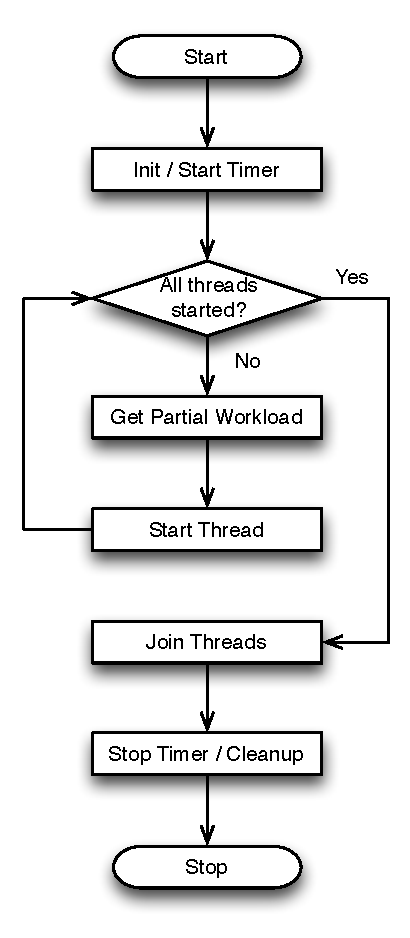
\includegraphics[width=0.85\textwidth]{figures/bench/host}
    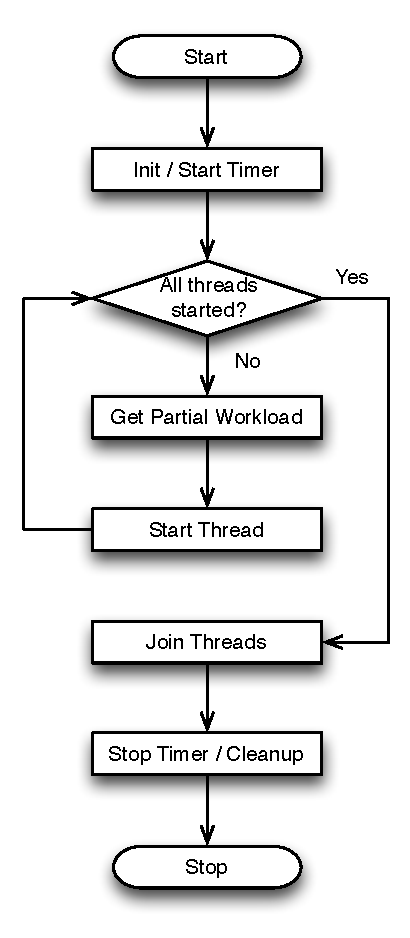
\includegraphics[width=0.75\textwidth]{figures/bench/host}
    \caption{Logical flow of the benchmark application.}
    \label{fig:eval-host}
\end{minipage}
\begin{minipage}[l]{0.50\textwidth}
    % 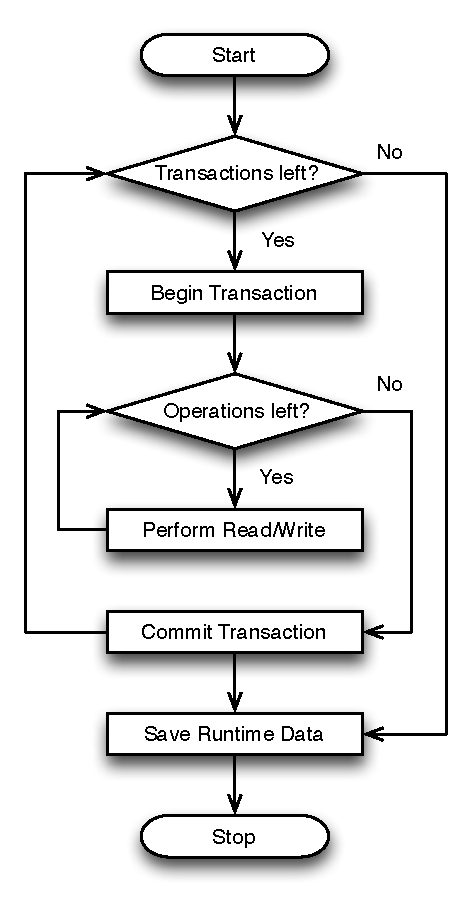
\includegraphics[width=\textwidth]{figures/bench/worker}
    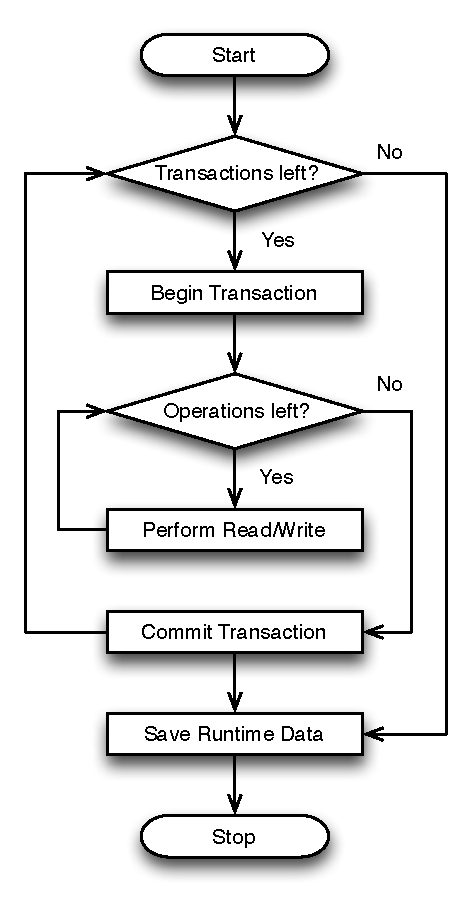
\includegraphics[width=0.89\textwidth]{figures/bench/worker}
    \caption{Logical flow of a single worker thread.}
    \label{fig:eval-worker}
\end{minipage}
\end{figure}

\subsubsection{Results \& Discussion}

\todo[inline]{Integrate raw ttp and parallel efficiency}

In this subsection the results of the benchmark are shown and discussed. The benchmark captures two metrics: transaction throughput and the transaction abort rate. In order to express the scalability of both KVS, throughput is expressed in terms of speedup factor. This also helps comparing the performance of both stores even if absolute throughput differs significantly. The abort rate is given by the ratio of the number of committed transactions and the number of scheduled transactions. When interpreting throughputs or speedup factors, it is important to take the abort rate into account because higher abort rates can lead to higher transaction throughputs. The reason for this circumstance is that commits are very expensive and the resulting time saving of an abort has a stronger influence on throughput than reducing the number of committed transactions. This is also a direct consequence of the two-level store architecture and the additional measures to preserve consistency in NVRAM.

\paragraph{Legend}

The following analysis compares benchmark results of Echo (green), Midas (blue) and an optimized variant of Midas (red). In the current implementation of Midas, the index is based on a naive hash table implementation for NVRAM. In order to protect critical sections in the hash table, a simple global locking mechanism is used. This approach forms a major bottleneck which can be addressed with a designated but often complicated concurrent design as in \cite{}. However, this is an implementation detail, albeit crucial. In order to show the potential of Midas' design, a second variant of Midas without index locking was examined. This is possible because during the benchmark not the index but only histories are modified. This is a side effect of omitting insert and delete operations for simplicity.

%==============================================================================
% [1 = SS]
%==============================================================================



\begin{figure}[h!]
\begin{minipage}[l]{0.50\textwidth}
    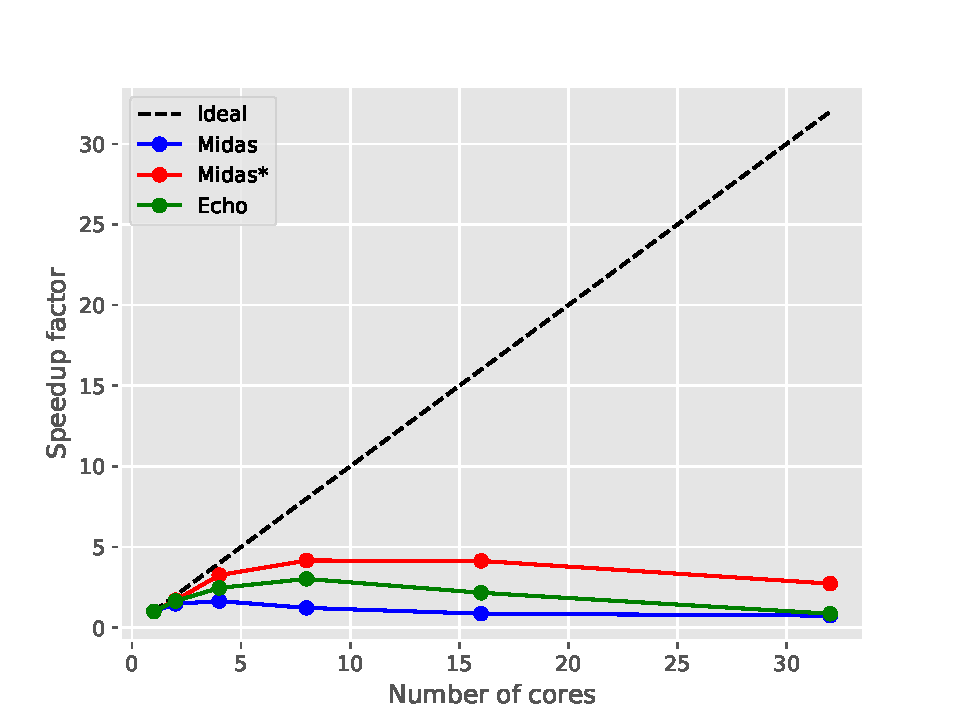
\includegraphics[width=\textwidth]{figures/bench/spd-ss}
    \caption{Transaction throughput speedup for scenario S1.}
    \label{fig:concept-two-level-store}
\end{minipage}
\begin{minipage}[l]{0.50\textwidth}
    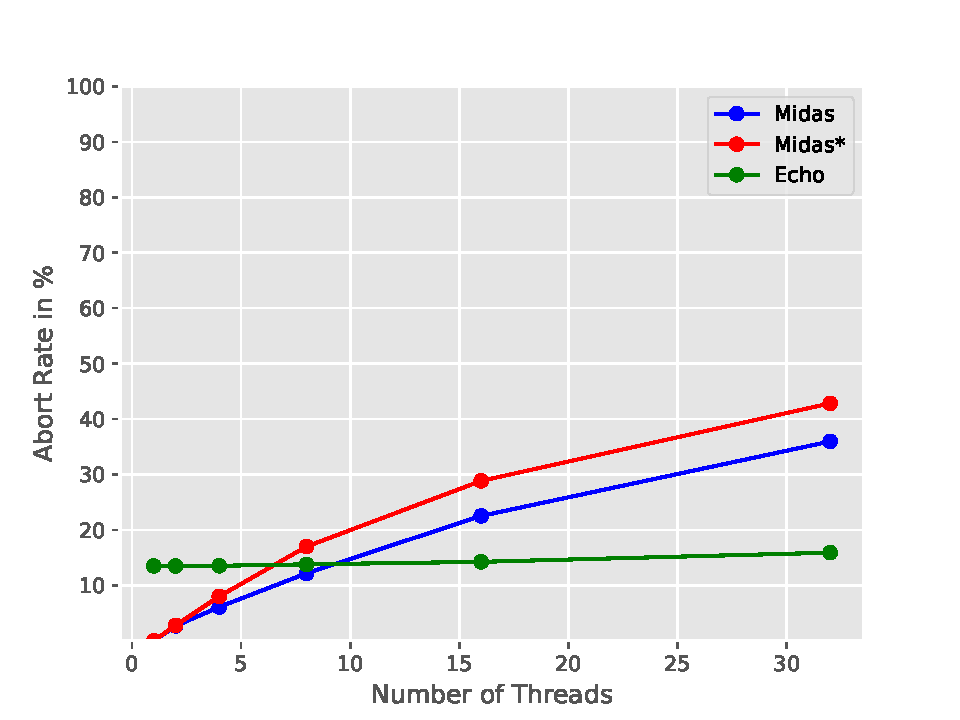
\includegraphics[width=\textwidth]{figures/bench/ar-ss}
    \caption{Abort rate for scenario S1.}
    \label{fig:concept-two-level-store}
\end{minipage}
\end{figure}

%==============================================================================
% [2 = SL]
%==============================================================================

\begin{figure}
\begin{minipage}[l]{0.50\textwidth}
        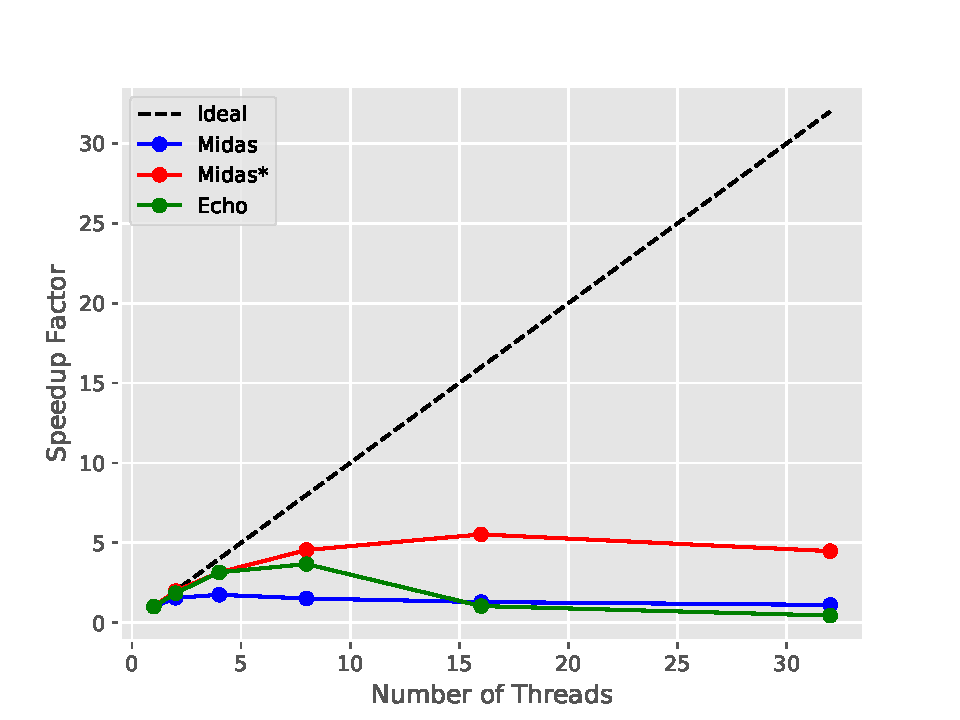
\includegraphics[width=\textwidth]{figures/bench/spd-ls}
        \caption{Transaction throughput speedup for scenario C}
        % \label{fig:concept-two-level-store}
    % \end{figure}
\end{minipage}
\begin{minipage}[l]{0.50\textwidth}
    % \begin{figure}
        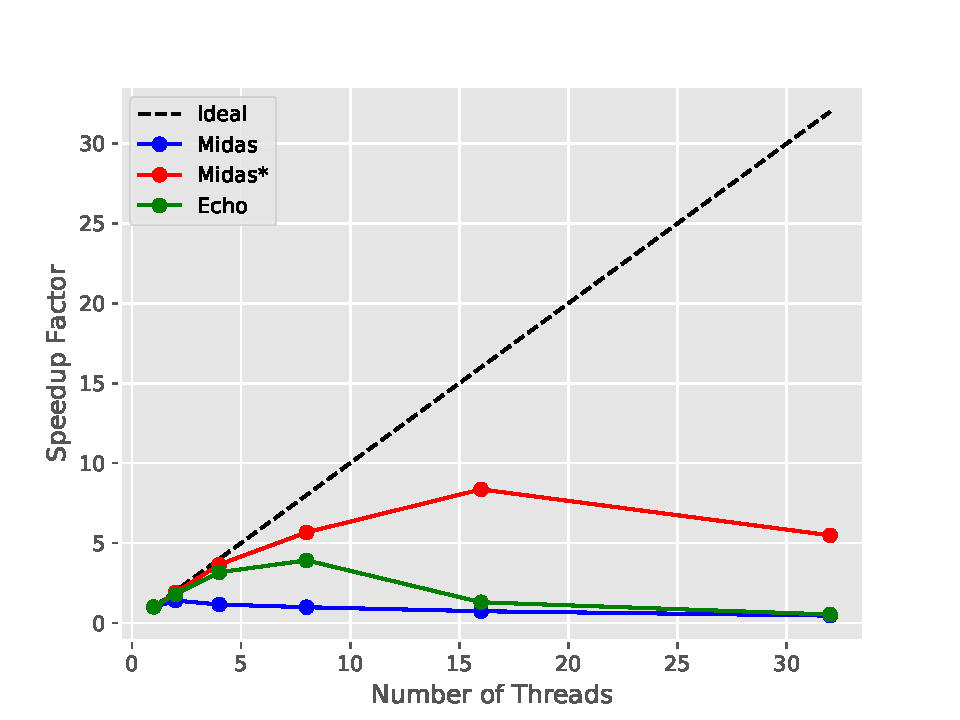
\includegraphics[width=\textwidth]{figures/bench/spd-ll}
        \caption{Transaction throughput speedup for scenario D}
        % \label{fig:concept-two-level-store}
\end{minipage}
\end{figure}

%==============================================================================
% [3 = LS]
%==============================================================================

\begin{figure}
\begin{minipage}[l]{0.50\textwidth}
        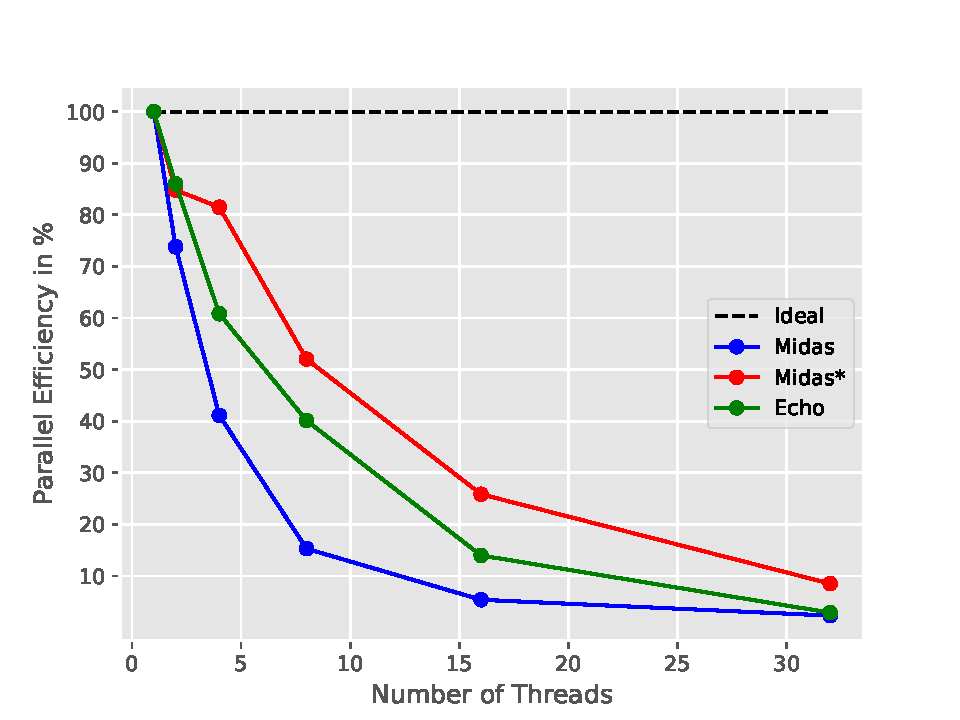
\includegraphics[width=\textwidth]{figures/bench/eff-ss}
        \caption{Parallel efficiency for scenario A}
        % \label{fig:concept-two-level-store}
\end{minipage}
\begin{minipage}[l]{0.50\textwidth}
    % \begin{figure}
        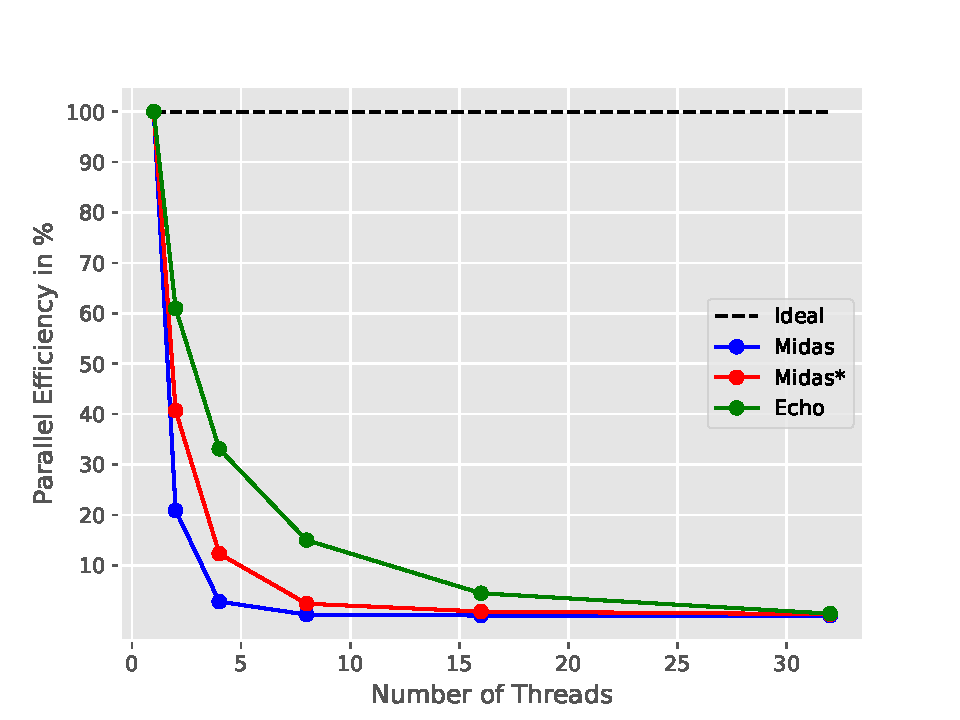
\includegraphics[width=\textwidth]{figures/bench/eff-sl}
        \caption{Parallel efficiency for scenario B}
        % \label{fig:concept-two-level-store}
    % \end{figure}
\end{minipage}
% \end{figure}

% \begin{figure}
\begin{minipage}[l]{0.50\textwidth}
        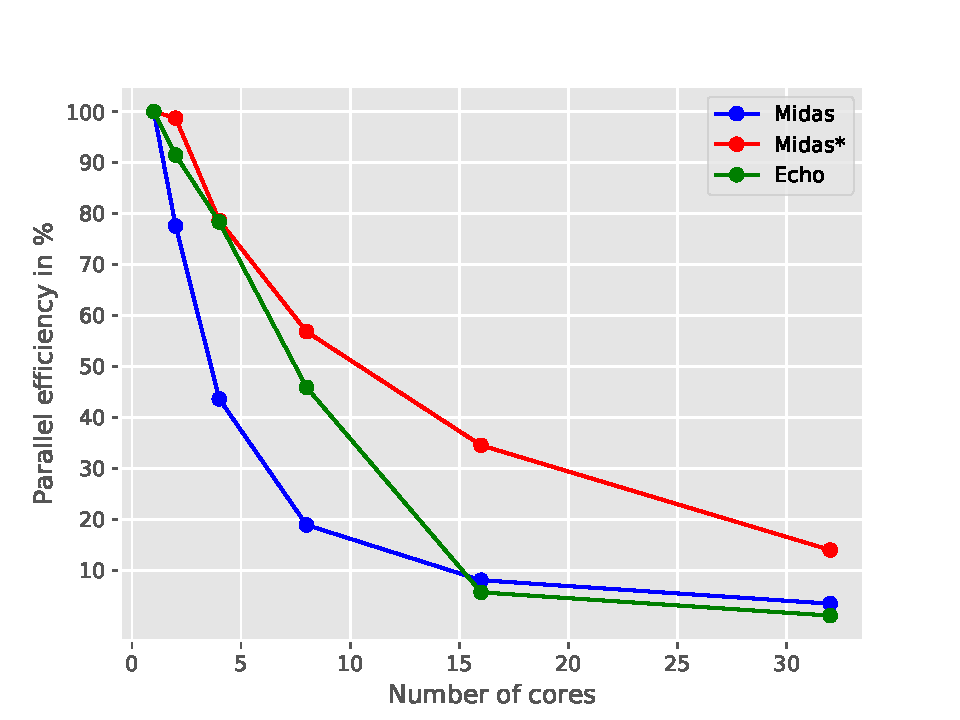
\includegraphics[width=\textwidth]{figures/bench/eff-ls}
        \caption{Parallel efficiency for scenario C}
        % \label{fig:concept-two-level-store}
    % \end{figure}
\end{minipage}
\begin{minipage}[l]{0.50\textwidth}
    % \begin{figure}
        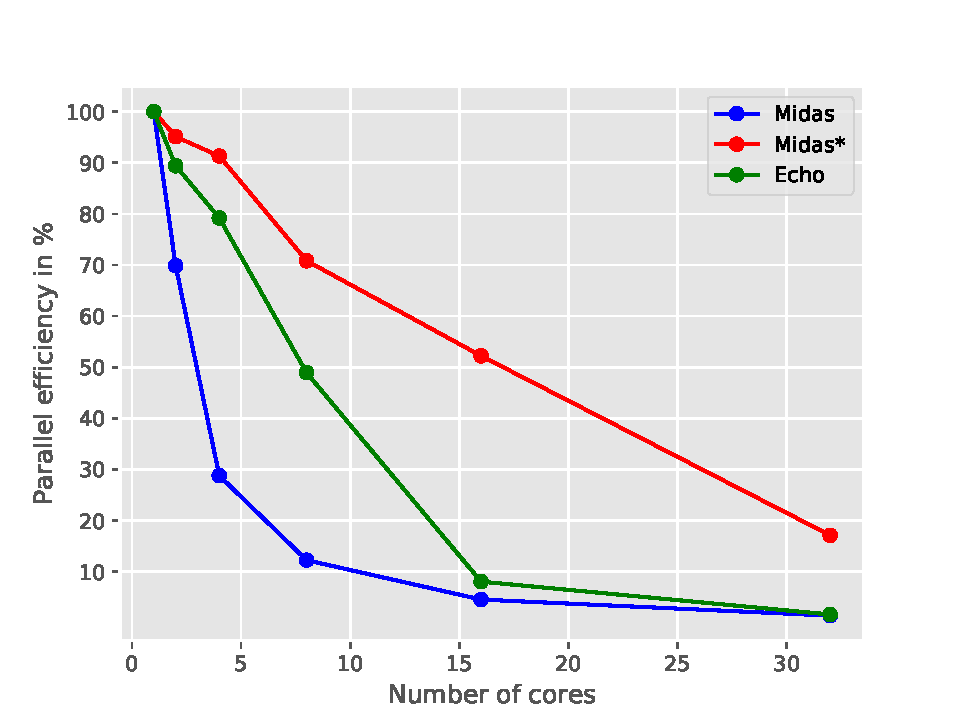
\includegraphics[width=\textwidth]{figures/bench/eff-ll}
        \caption{Parallel efficiency for scenario D}
        % \label{fig:concept-two-level-store}
\end{minipage}
\end{figure}

%==============================================================================
% [4 = LL]
%==============================================================================

\begin{figure}
\begin{minipage}[l]{0.50\textwidth}
        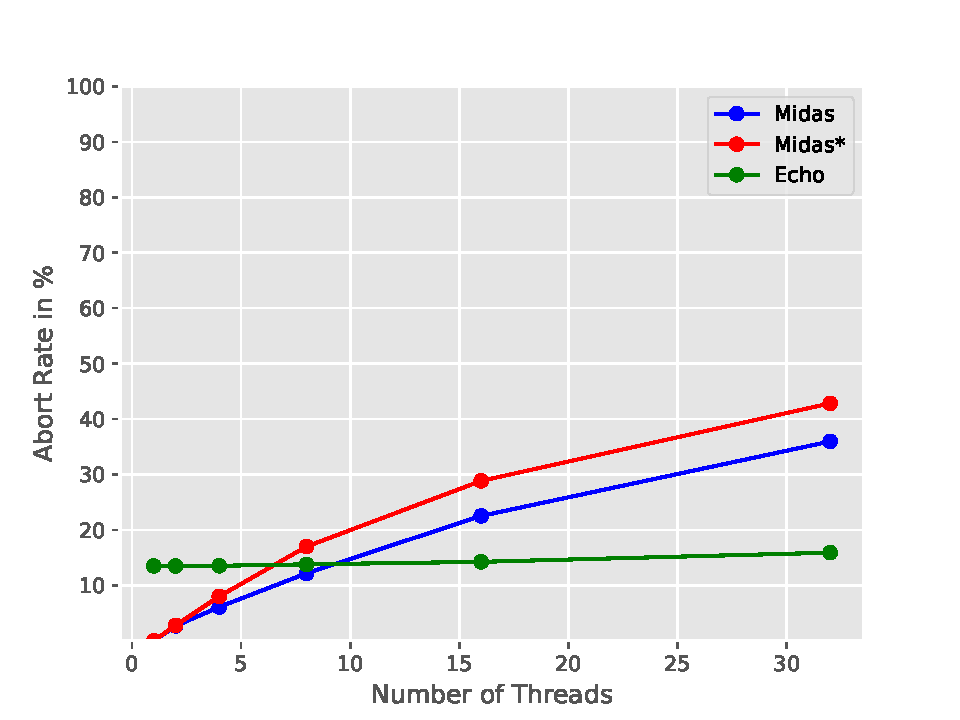
\includegraphics[width=\textwidth]{figures/bench/ar-ss}
        \caption{Abort rates for scenario A}
        % \label{fig:concept-two-level-store}
\end{minipage}
\begin{minipage}[l]{0.50\textwidth}
    % \begin{figure}
        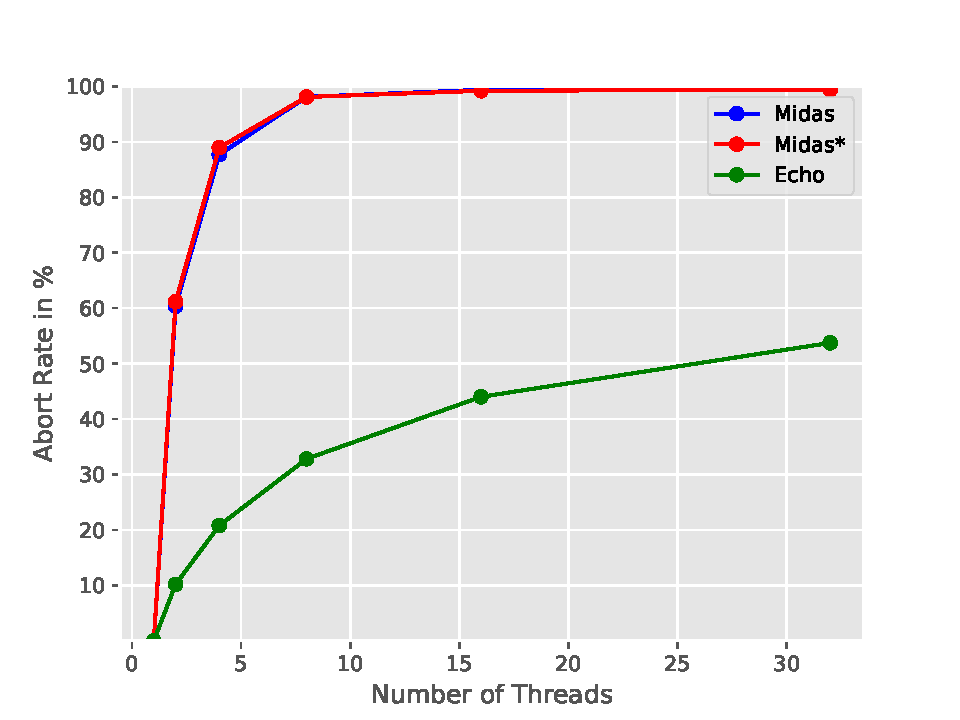
\includegraphics[width=\textwidth]{figures/bench/ar-sl}
        \caption{Abort rates for scenario B}
        % \label{fig:concept-two-level-store}
    % \end{figure}
\end{minipage}
% \end{figure}

% \begin{figure}
\begin{minipage}[l]{0.50\textwidth}
        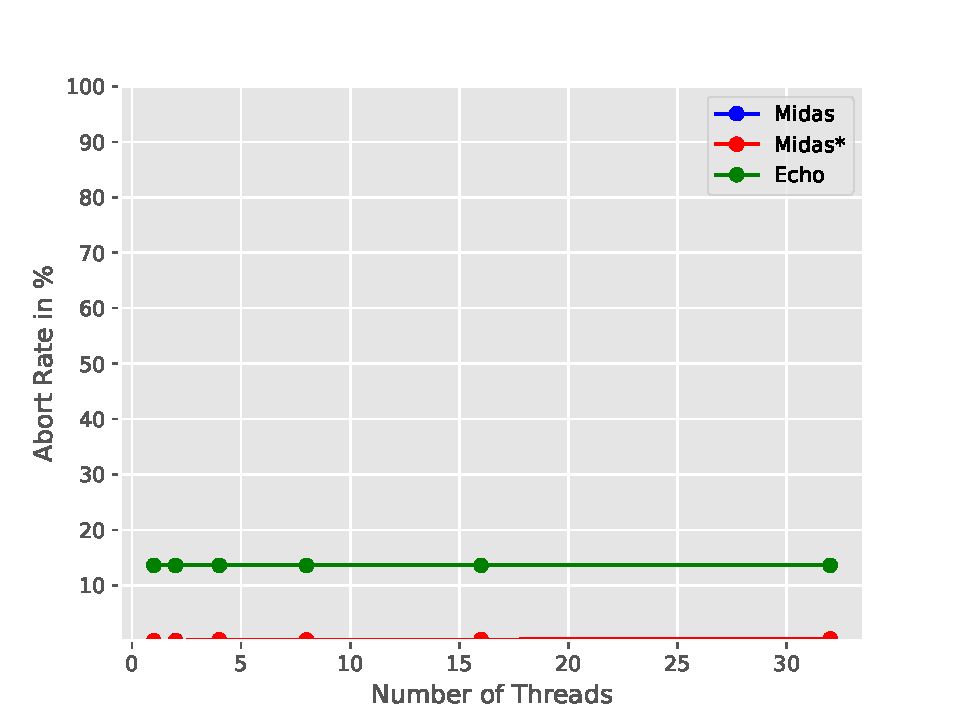
\includegraphics[width=\textwidth]{figures/bench/ar-ls}
        \caption{Abort rates for scenario C}
        % \label{fig:concept-two-level-store}
    % \end{figure}
\end{minipage}
\begin{minipage}[l]{0.50\textwidth}
    % \begin{figure}
        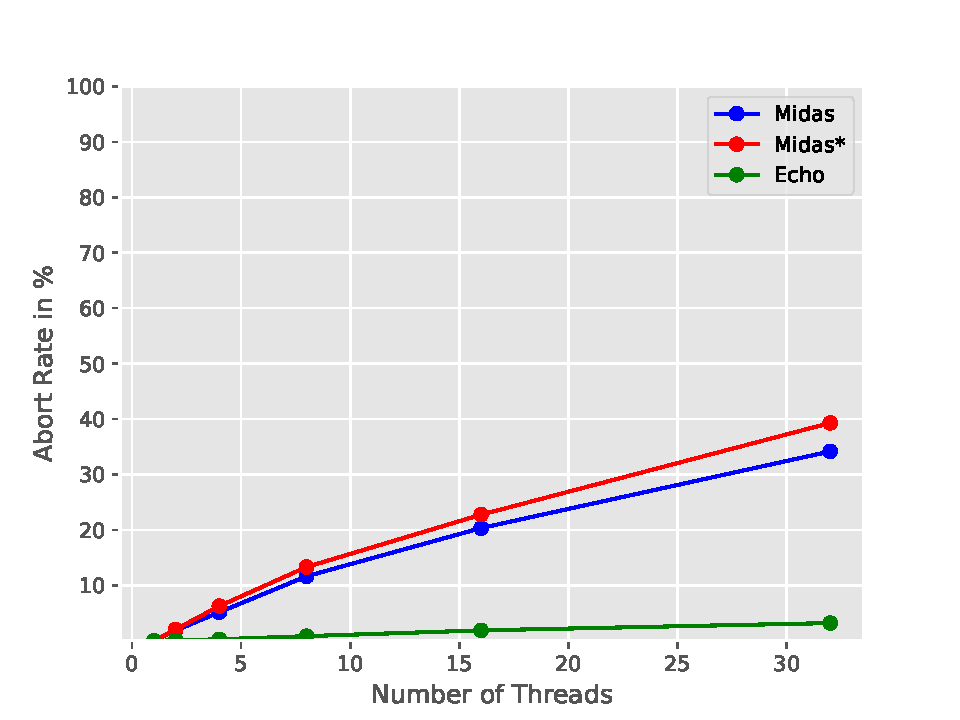
\includegraphics[width=\textwidth]{figures/bench/ar-ll}
        \caption{Abort rates for scenario D}
        % \label{fig:concept-two-level-store}
\end{minipage}
\end{figure}

\todo[inline]{Werden Captions mit Punkt beendet???}
